\begin{table*}[htbp!]
	\centering
	\caption{Query Features and information on their range and correlations with other (discarded) features.}
	\label{table:features}
	%\scalebox{0.9}{
	\begin{tabular}{l|llll}
		\hline
		\textbf{Feature} & \textbf{Prefix} & \textbf{Value} & \textbf{Range} & \textbf{Correlations} \\
		\hline
		\sql{order}       & ORD     & frequency  & [0,1]   & \sql{limit}(0.88) \\
		\sql{filter in}   & FIL\_IN & frequency  & [0,16]  & \sql{union}(0.95), FS(0.95) \\			
		\sql{filter}      & FIL     & frequency  & [0,27]  & tp\_???(0.96), TP(0.95) \\
		\sql{count}       & CNT     & frequency  & [0,1]   & \sql{distinct}(1.0) \\
		Triple Patterns   & TP      & frequency  & [1,38]  & \sql{filter}(0.95) \\
		\sql{graph}       & GRA     & frequency  & [0,1]   & - \\
		\sql{optional}    & ORD     & frequency  & [0,9]   & - \\
		\sql{group}       & GRP     & frequency  & [0,4]   & - \\
		(sub)Queries      & Q       & frequency  & [1,10]  & \sql{union}(0.94), \sql{filter in}(0.94) \\
		file size         & FS      & kilobyte  & 1, 10, 100  & \sql{filter in}(0.97), \sql{union}(0.95) \\
		query engine      & -      &  \emph{Vendor}  & -  & - \\
		\hline
	\end{tabular}
	%}
\end{table*}

\begin{figure*}[htbp!]
	\centering
	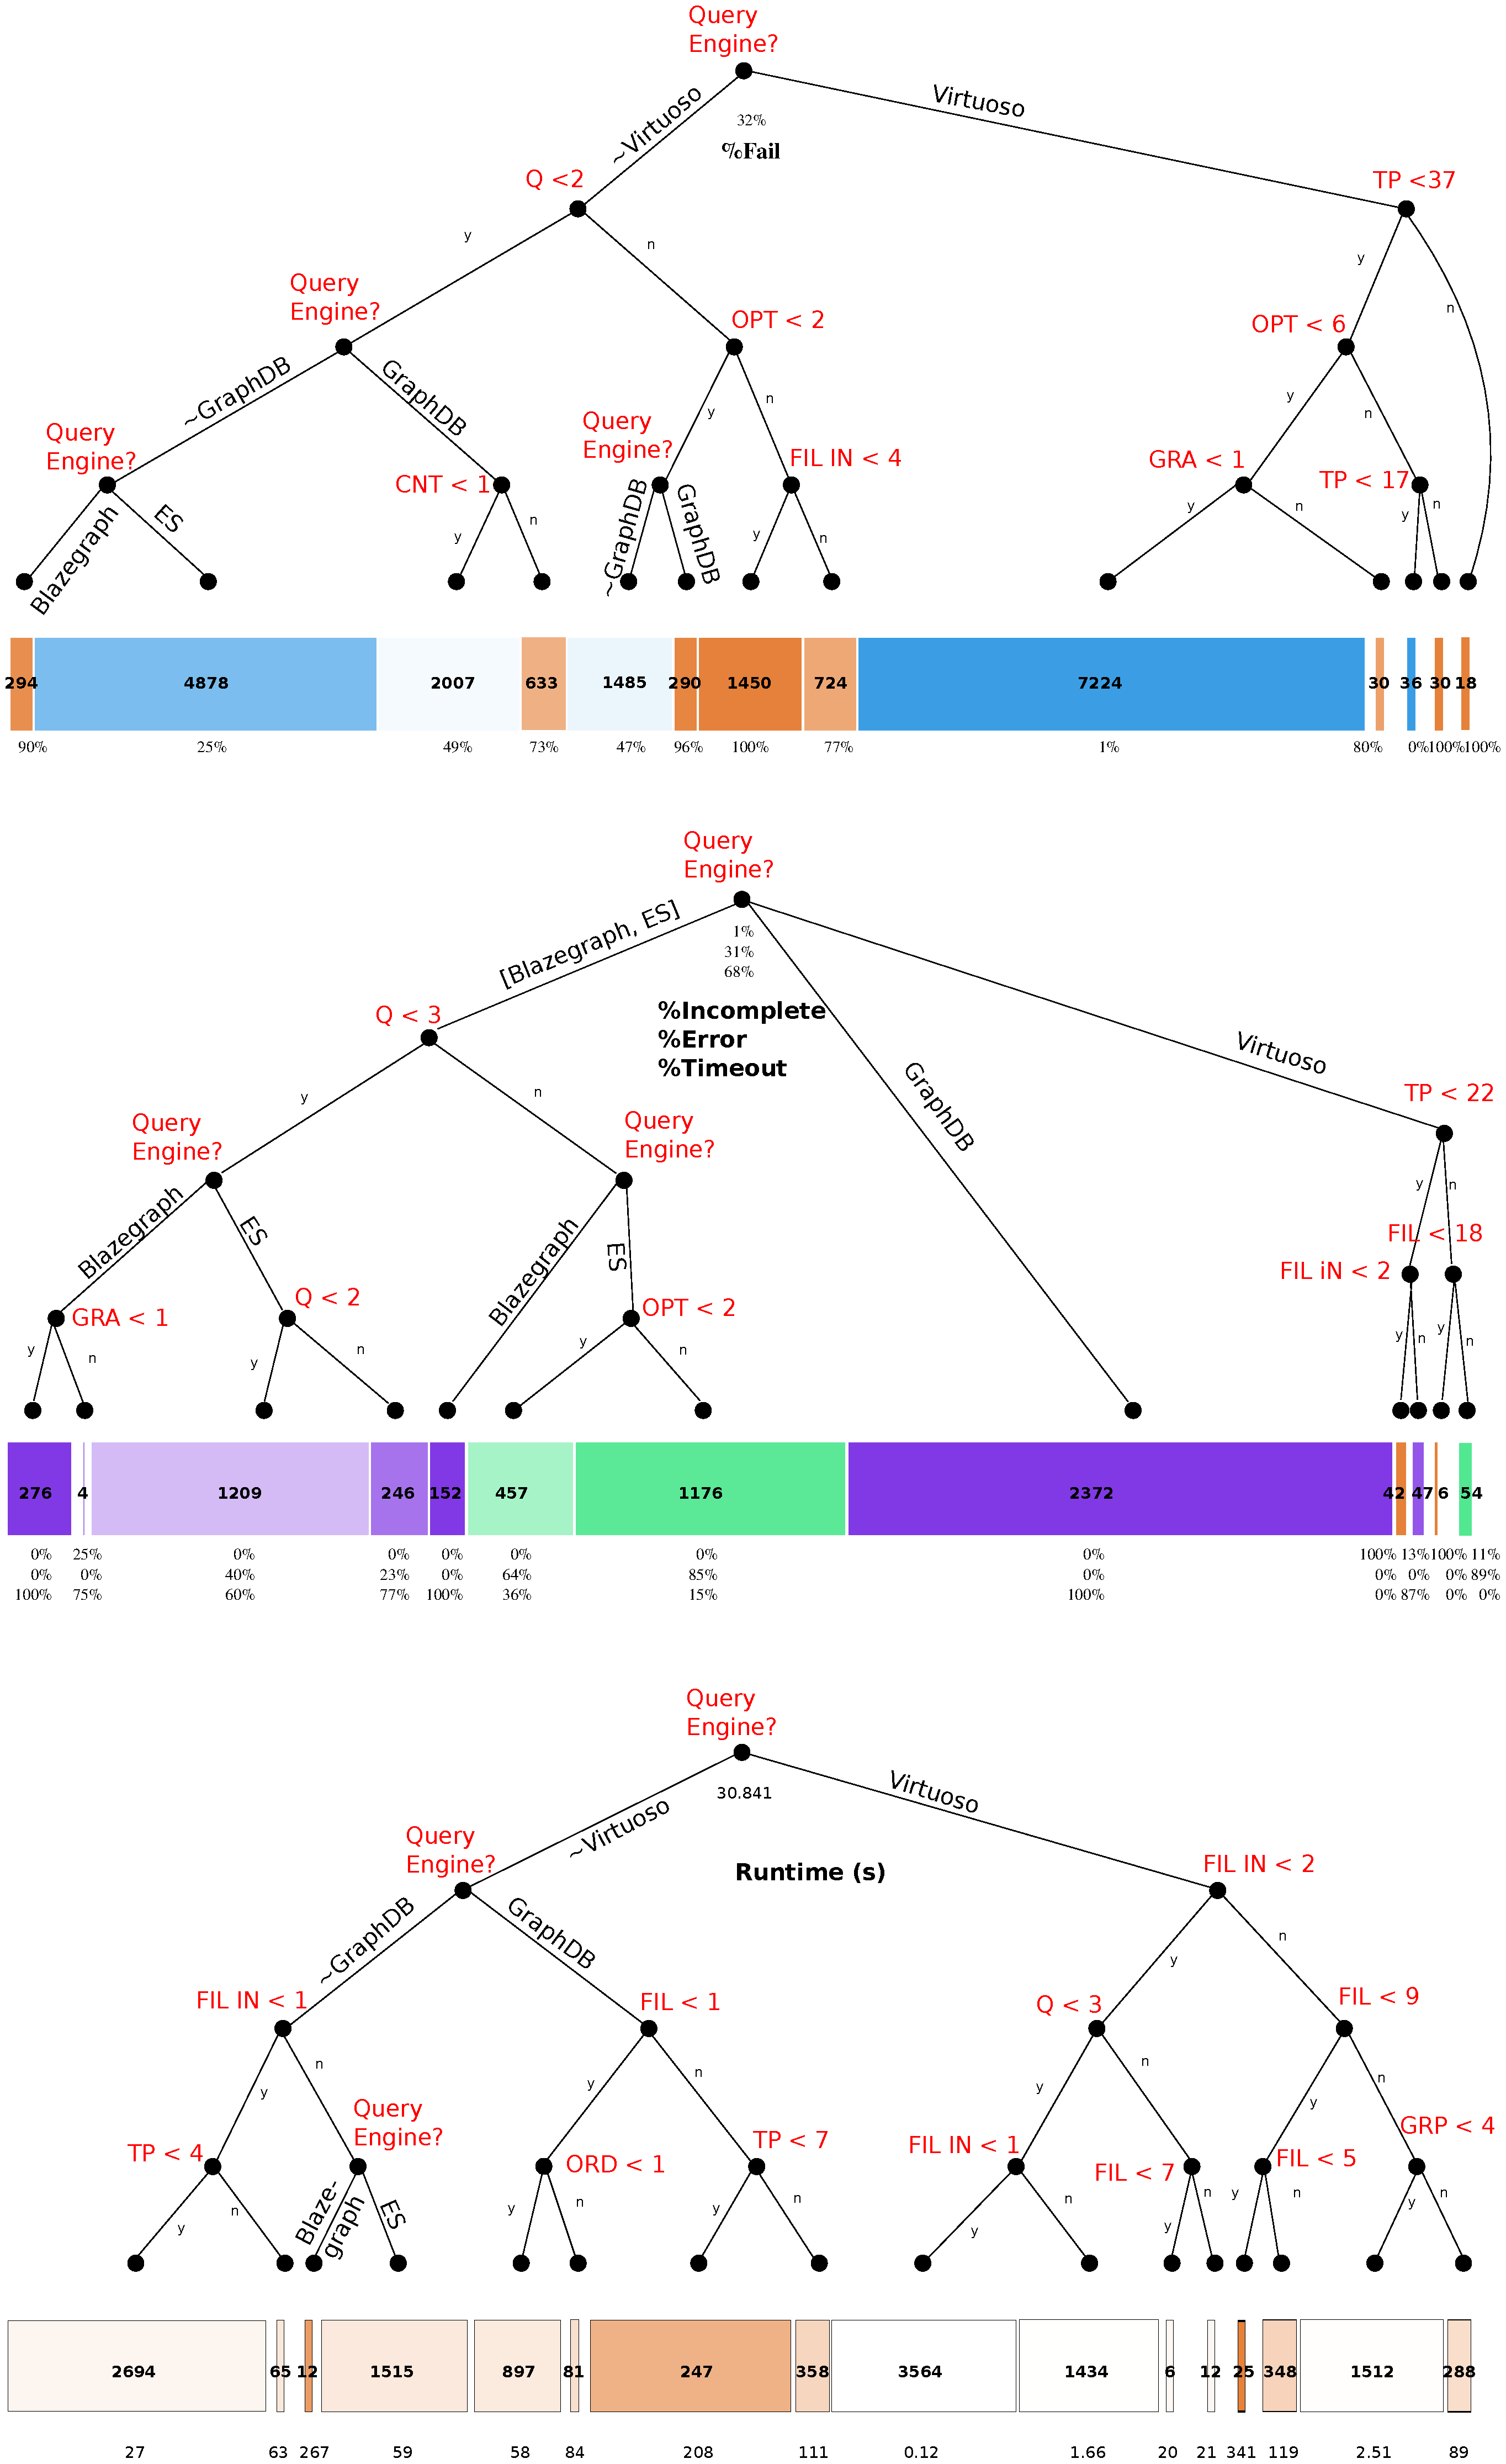
\includegraphics[width=0.75\linewidth]{imgs/Fig10_AllTrees}
	\caption{Decision Tree Analysis to identify the reason for query failure, certain error types, and high/low query runtimes. Input for all trees are feature vectors, also the query engine is added as a categorical feature. Rules in the decision trees are shown in red, sample sizes are encoded as the width of the bottom bar and the value is added inside the bars in bold. For each separate part the class distribution or the average runtime is reported below the bar. 
	\newline \hspace{\linewidth} 	
	\underline{\smash{Top:}} Classification into query success (blue) and failure (red) and incomplete. The query engine is an important decision rule, which demonstrates that Virtuoso behaves very different from the other systems.  
	\newline \hspace{\linewidth} 	
	\underline{\smash{Center:}} Classification of query failures into classes incomplete (orange), server error (green), and timeout (purple). 
	\newline \hspace{\linewidth} 	
	\underline{\smash{Bottom:}}  Regression on query runtimes. Red corresponds to high query runtimes, white to low. }
 	\label{fig:Fig10_AllTrees}
\end{figure*}


%

%	\caption{Decision Tree Analysis to identify the reason for query failure, certain error types, and high/low query runtimes. Input for all trees are feature vectors which represent the frequencies of operators and some structural features such as the amount of sub-queries. Also the query engine is added as a categorical feature. Rules in the decision trees are shown in red, sample sizes are encoded as the width of the bottom bar and the value is added inside the bars in bold. For each separate part the class distribution or the average runtime is reported below the bar. \\ 
%		\textbf{Top:} Classification into query success (blue) and failure (red) and incomplete.  
%		The query engine is an important decision rule, which demonstrates that Virtuoso behaves very different from the other systems. For those (left hand side), the amount of sub-queries (Q) and \sql{optional}s play a big role in predicting query failure. \\
%		\textbf{Center:} Classification of query failures into classes incomplete (orange), server error (green), and timeout (purple). \textbf{Gra1} and \textbf{Bla1} only have timeouts. \textbf{ES1} has a large fraction of HTTP errors as well. \\
%		\textbf{Bottom:}  Regression on query runtimes. Red corresponds to high query runtimes, white to low. For \textbf{Vir1} the amount of \sql{filter in} and \sql{group} (GRP) operators are the most important factors. \textbf{Gra1} seems to run slower for queries containing \sql{filter} (FIL) operators. For the other two systems the presence of \sql{filter in} affects the runtimes negatively.
%		\\
%	}




Ontoforce has released the queries for this benchmark run. However, the queries are very complex and sometimes they take up 1 - 100 kb in disk space. To gain a deeper understanding into why queries fail, have timeouts and HTTP errors, why they are fast or slow to execute,... we created a set of features per query and fitted a decision tree~\footnote{\scriptsize \url{http://scikit-learn.org/stable/modules/tree.html}} to the data. The 3 resulting trees are shown in Figure~\ref{fig:Fig10_AllTrees}. The input features for this algorithm are limited by removing highly correlated features. For example \sql{order} and \sql{limit} are highly correlated. The list of retained query features is given in Table~\ref{table:features} together with the highest correlated operators.
By adding `Query Engine' as an additional feature we can train the decision tree on all the available query event data for the Ontoforce Benchmark. 
\begin{itemize}
	\item \textbf{Dominant Feature:} The `Query Engine' is the most important factor to segment the data in all 3 cases. The absence of this feature would in fact indicate that all systems have similar behaviour. \textbf{Vir1} thus is very different: it has fewer errors and query runtimes are significantly smaller.
	\item \textbf{Feature Importance:} If we take the number of node occurrences as a feature as a measure for feature importance then we see 3 features which occur in 5 nodes: TP, \sql{filter in}, \sql{filter}. The \sql{filters} mainly play a role in the decision tree for runtime regression. In predicting failures and error types \sql{optional}, \sql{graph} and Q have the higest occurrences.
	%Fail: Engine:4    Q:1 TP:2, OPT:2, GRA:1, FILIN:1, FIL:0
	%Error: Engine:3   Q:2 TP:1, OPT:1, GRA:1, FILIN:1, FIL:1
	%SUBTOTAL: Engine:7  Q:3 TP:3, OPT:3, GRA:3, FILIN:2, FIL:1, ORD:0, GRP:0  
	%Runtime: Engine:3 Q:1 TP:2, OPT:0, GRA:0, FILIN:3, FIL:4, ORD:1, GRP:1 
	%TOTAL: Engine:10  Q:4 TP:5, OPT:3, GRA:3, FILIN:5, FIL:5, ORD:1, GRP:1  
	\item \textbf{Highest failure rates:} The paths leading to samples with a high failure rate generally contain \sql{optional} operators. All engines except for \textbf{Vir1} suffer when $Q > 1$. \textbf{Gra1} also has a high failure rate for \sql{count} queries.
	\item \textbf{Most frequent error types:} For \textbf{Bla1} and \textbf{Gra1} the errors are all timeouts (purple). For \textbf{ES1} having multiple subqueries often leads to HTTP errors (green). 
	\item \textbf{Queries with high runtimes:} For \textbf{Vir1} and \textbf{ES1} the \sql{filter in} operators are the main cause for high runtimes. For \textbf{Gra1} the presense of \sql{filter}s pushes runtimes above 100s. 
\end{itemize}

Finally we also investigate if the incorrect queries in the \textbf{Vir3} benchmarks had specific query features. Curiously, the problematic queries correspond to the most simple queries: $TP \leq 2$.	
